\documentclass[]{standalone}

\usepackage{amsmath}
\usepackage{amsfonts}
\usepackage{amssymb}
\usepackage{graphicx}
\usepackage{tikz}
\usepackage{import}
\usepackage[subpreambles=true]{standalone}

\usepackage{tikz}
\usepackage{tikz-3dplot}

\usetikzlibrary{calc}
\usetikzlibrary{positioning}

\begin{document}

    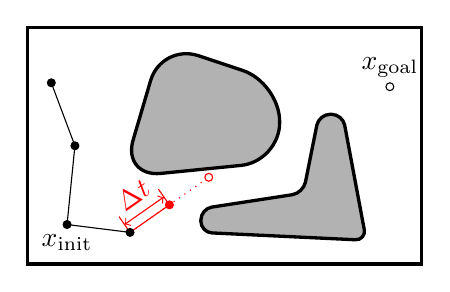
\begin{tikzpicture}[scale=1]

        \useasboundingbox (0,0) rectangle (5,3);

        \coordinate (init) at (0.5,0.5);
        \coordinate (goal) at (4.6,2.25);
        \coordinate (obs1) at (2.4,2.1);
        \coordinate (obs2) at (3.7,0.65);

        \coordinate (n0) at (0.6, 1.5);
        \coordinate (n1) at (0.3, 2.3);
        \coordinate (n2) at (1.3, 0.4);
        \coordinate (sample) at (2.3, 1.1);
        \coordinate (addedpoint) at ($(n2)+0.5*(sample)-0.5*(n2)$);

        \path[draw, fill] (init) circle (0.05) node[below] {$x_\mathrm{init}$};
        \path[draw] (goal) circle (0.05) node[above] {$x_\mathrm{goal}$};

        \path[draw, very thick] (0,0) -- (5,0) -- (5,3) -- (0,3) -- cycle;

        \path[draw] (init) -- (n0) -- (n1);
        \path[draw] (init) -- (n2);

        \path[draw, red, dotted] (n2) -- (sample);
        \path[draw, red] (n2) -- (addedpoint);


        \path[draw, red] (n2) -- ($(n2)!0.4!90:(addedpoint)$);
        \path[draw, red] (addedpoint) -- ($(addedpoint)!0.4!90:(sample)$);
        \path[draw, <->, red] ($(n2)!0.2!90:(addedpoint)$) -- ($(addedpoint)!0.2!90:(sample)$) node [midway, above, sloped] {$\Delta t$};

        \foreach \x in {0,...,2}
            \path[draw, fill] (n\x) circle (0.05);

        \path[draw=red, fill=white] (sample) circle (0.05);
        \path[draw, fill, red] (addedpoint) circle (0.05);

        \path[draw, very thick, rounded corners=14pt, fill=black!30] (obs1) ++(-1.2,-1) -- ++(2,0.2) -- ++(0,1) -- ++(-1.5,0.5) -- cycle;
        \path[draw, very thick, rounded corners=4pt, fill=black!30] (obs2) ++(-1.5,-0.25) -- ++(0,0.3) -- ++(1.3,0.2) -- ++(0.2,1) -- ++(0.3,0) -- ++(0.3,-1.6) -- cycle;

    \end{tikzpicture}
\end{document}